\section{Conclusion and future work} \label{sec:conclusion}

In this paper, a brief overview of the exploration strategies in both 2d and 3D spaces is given. A modular approach to autonomous decentralized multi-robot exploration and mapping was presented. Even though the strategy achieved our expectations, the algorithm is open towards improving. Future research should consider decentralized map creating weather by integration with a developed approaches or proposing a new one. Given this state-of-the art overview, one research direction can be an extension to the algorithm to cope with a limited communication range of the robots.

This paper presents a solution to autonomously explore 3D environment without requiring an initial map. Octomap itself is able to handle dynamic environments by updating the map (in parallel with SLAM) which makes the algorithm works well in dynamic environment.
If we consider 3D exploration, an extension to multi aerial vehicles coordination algorithm can be a significant improvement. Also, if we take a map sharing of each robot to others into consideration, we can improve out trajectory planner and avoid many robots go on same paths in different times. Finally, we would like to take into consideration scenarios in which the robots may fail as well as time-varying environment scenarios.

To conclude, this work is a stepping stone for new research in coordinated multi-robot exploration algorithms and its decentralization.

\begin{figure}[t]
	\centering
	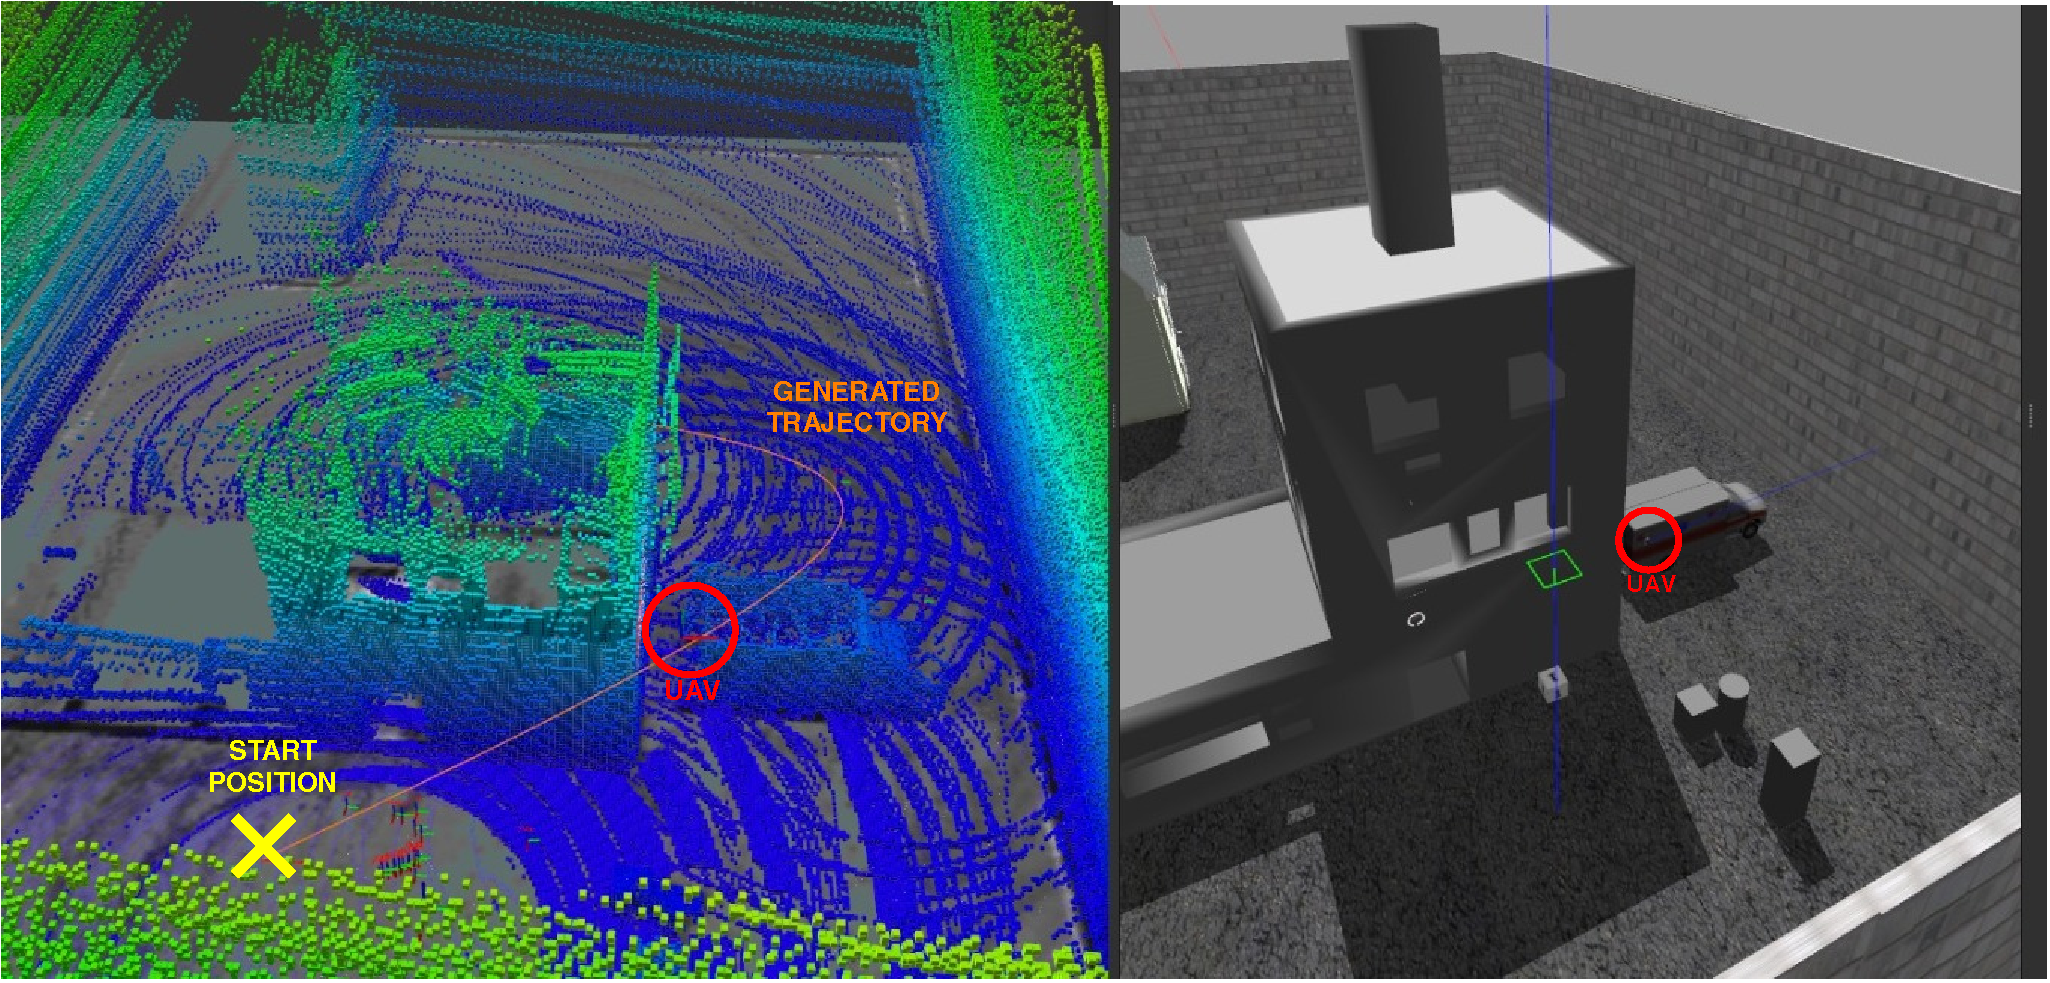
\includegraphics[width=1.0\columnwidth]{./pictures/rviz_gazebo.pdf}	
	\caption{UAV is executing generated trajectory.}
	\label{fig:rviz_gazebo}
\end{figure}